\section{Configuração de uma Rede}

\subsection{Experiência 1}

Nesta experiência configuraram-se endereços IP de duas máquinas ligadas através de um switch para entender melhor como funciona a comuniação entre máquinas e o significado e funcionamento de pacotes ARP.

\begin{figure}[!h]
\centering
  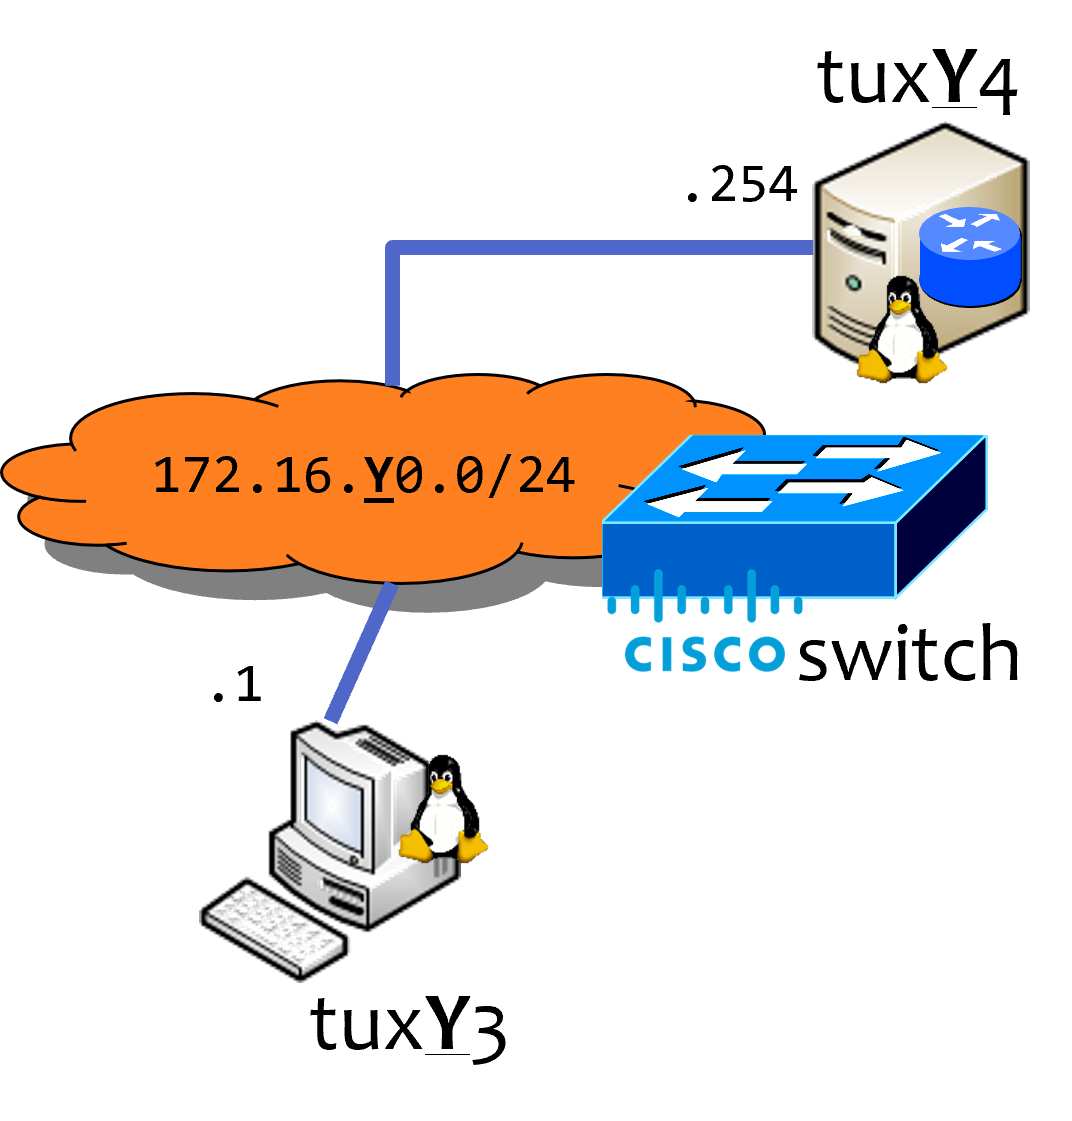
\includegraphics[width=.3\linewidth]{img/exp1-net.png}
  \caption{Estrutura da rede}
\end{figure}

\subsubsection{Questões}

\paragraph{O que são os pacotes ARP e para que são usados?}
Os pacotes do protocolo ARP são utilizados para, sabendo o endereço IP de uma maquina, descobrir o seu endereço MAC. 

\paragraph{O que são os endereços MAC e IP dos pacotes ARP e porquê?}
Os endereços MAC identificam as interfaces com a rede que uma determinada máquina utiliza para comunicar com outras máquinas. Nos pacotes ARP utilizados para pedir o endereço MAC da interface de uma máquina, o primeiro endereço é enviado para que se identifique o endereço IP da máquina cujo endereço MAC é procurado. O segundo é utilizado para identificar a máquina que pretende ser informada. Nos pacotes ARP de resposta, o primeiro endereço IP é enviado para identificar a máquina que possui o endereço MAC enviado em segundo lugar.

\paragraph{Que pacotes gera o comando PING?}
São gerados pacotes ICMP utilizados para mandar erros da camada 3 ou mensagens para routers. Neste caso são utilizados para testar a conectividade entre as máquinas da rede.

\paragraph{Quais são os endereços IP e MAC dos pacotes de PING?}
O endereço IP de origem dos pacotes enviados é 172.16.50.1, o endereço do tux53. O endereço IP de destino é 172.16.50.254, o endereço de IP do tux54.  O endereço MAC de origem dos pacotes é 00:21:5a:61:2d:72 o endereço de eth0 do tux53. O endereço MAC de destino é 00:21:5a:c3:78:70, o endereço de eth0 do tux54. 

\paragraph{Como determinar se um frame Ethernet recebido é ARP, IP, ICMP?}
Ao analisar os pacotes no Wireshark pode verificar-se o tipo de frame analisando os bytes 12-13 do pacote recebido. Os pacotes ARP têm tipo 0x0806 os pacotes IP têm tipo 0x0800. Os pacotes ICMP têm o mesmo tipo dos pacotes IP e o byte 23 é 0x01. O Wireshark faz esta análise portanto basta ver a coluna Protocol para cada pacote.

\paragraph{Como determinar o comprimento da trama recebida?}
O comprimento das tramas pode ser observado no Wireshark na coluna Length. As tramas IP possuem o seu tamanho nos bytes 16-17.

